\documentclass[12pt]{iopart}
\usepackage{graphicx}
%\usepackage{witharrows}
\usepackage{extarrows}
\usepackage{mathtools}
\usepackage{amssymb}
\usepackage{units}
\usepackage{tabto}
\usepackage{subfig}
\usepackage{ntheorem}
\theoremstyle{break}
\newtheorem{prop}{Definition}[section]
\counterwithin{equation}{section}
\DeclareMathOperator{\E}{\mathbb{E}}
\DeclareMathOperator{\sign}{sign}
\newcommand*{\QEDA}{\null\nobreak\hfill\ensuremath{\diamond}}%
\newcommand*{\QEDB}{\null\nobreak\hfill\ensuremath{\blacksquare}}%
\newcommand*{\sfig}[2]{\begin{figure}[htpb]\centering\subfloat[#2]{\includegraphics[width=1.0\linewidth]{#1}}\end{figure}}
\bibliographystyle{iopart-num}
\begin{document}
\date{February 2023}
\title{Notes on the Forward-Forward Algorithm}
\author{Akhil Sadam$^1$, Dr.Tan Bui Thanh$^2$}
\address{$^1$Department of Aerospace Engineering and Engineering Mechanics, UT Austin\\$^2$The Oden Institute for Computational Sciences, UT Austin}
\ead{akhil.sadam@utexas.edu, tanbui@oden.utexas.edu}
\begin{indented}
\item[]February 2023
\end{indented}
\section{Motivation}
This document primarily derives missing formulas from Dr. Hinton's paper \cite{FFA23}, providing a more rigorous framework for further investigation.
Note that the Forward-Forward Algorithm (FFA) performs only classification.
\section{Base Forward-Forward Architecture (Supervised)}
Assume a supervised problem with $m$ labels and $t$ test samples as below.
\begin{alignat}{2}
\mathbf{X_{test}} = \{x_i \mid i \in 1,...,t \},\ \mathbf{Y_{labels}} = \{y_j \mid j \in 1,...,m \}
\end{alignat}

\begin{figure}[htpb]
\centering

\subfloat[Supervised FFA Architecture]{
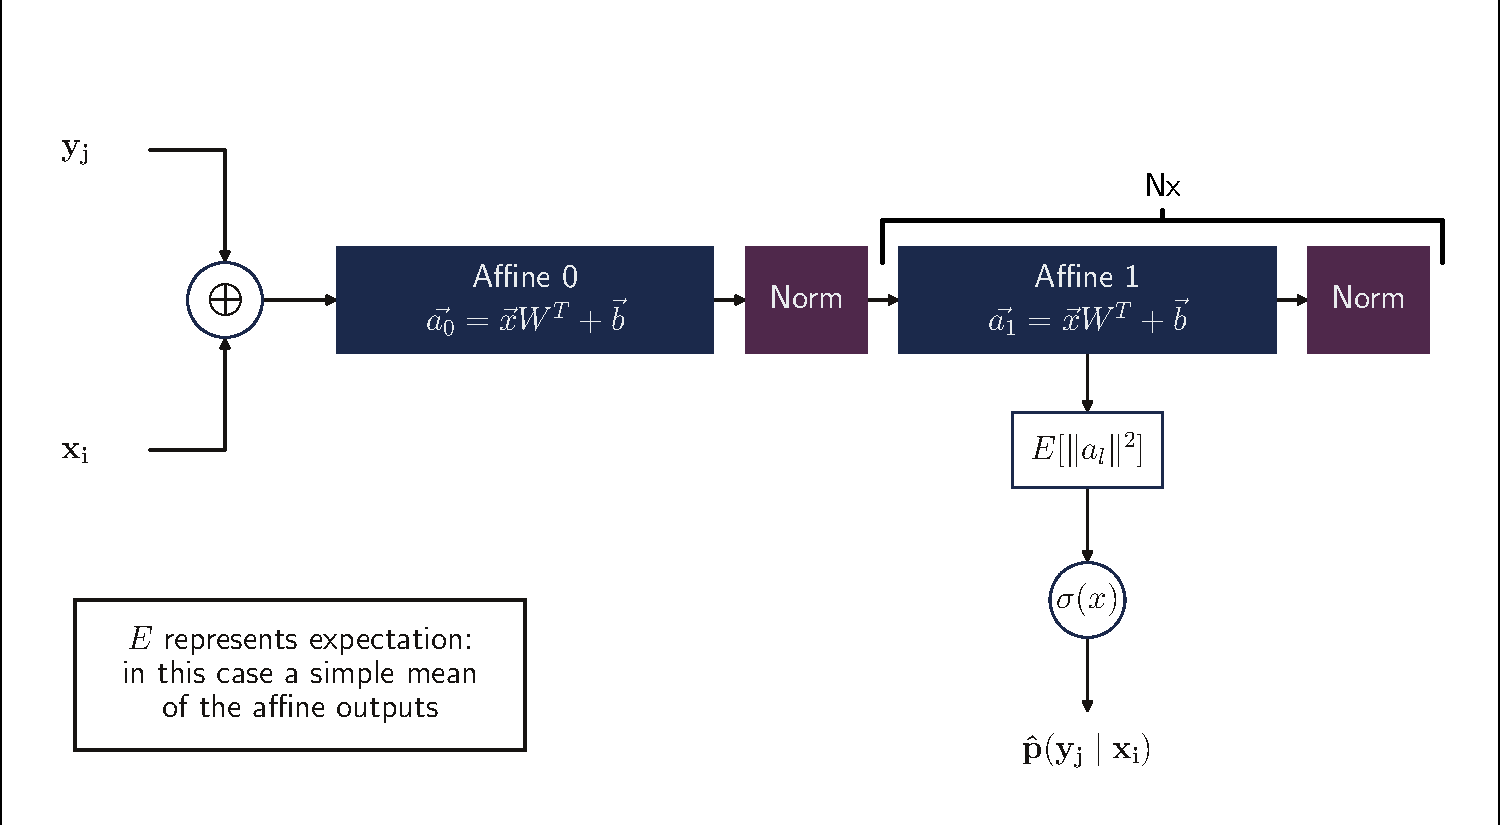
\includegraphics[width=0.8\linewidth]{FFA/memo/code//../plots/ffasup}
\label{fig:ffasup}
}

\end{figure}

In prediction mode, each test sample $x_i$ is combined with every label $y_j, \forall j\in 1,...,m$. The net [Fig.~\ref{fig:ffasup}] outputs $m$ predictions of $\hat{p}(y_j \mid x_i)$.
For a single-label classifier, the label with the highest probability is chosen.
To classify all samples the FFA requires $m*t$ runs.
Normalization is required after each layer to ensure that prior layer $\|a_{l-1}\|^2$ does not affect later layers.
Training is a greedy layer-by-layer approach.
\section{FFA Training}
\fbox{$a_{l-1}$ will represent $a_{l-1}^{norm}$ in this section, as only one layer is considered.}\\
\subsection{Loss Derivation}
Consider a single layer of the FFA. Note the following:
\begin{description}\item
Each layer is trained to predict $\hat{p}(y_j \mid x_i)$ from $a_{l-1}$.
Training data consists of two datasets, assuming $n$ known points $(x_i,y_i)$.
\begin{alignat}{2}
\mathbf{D_{+}} &:= \{(x_{+i},y_i) \mid i \in 1,...,n \} := \{(x_i,y_i) \mid i \in 1,...,n \} \\
\mathbf{D_{-}} &:= \{(x_{-i},y_i) \mid i \in 1,...,n \} := \{(x_i*,y_i) \mid i \in 1,...,n \}
\end{alignat}
The positive dataset is simply the correctly labeled points. The negative dataset is defined as incorrectly-labeled or corrupted data; the FFA paper \cite{FFA23} does not identify a best choice.
Notice also that the negative dataset need not be the same size as the positive dataset, just a scalar multiple.
The later implementation uses $x_i*$ as a random sample (taking exactly one negative sample per datapoint).
\begin{alignat}{2}
x_i* \in \{x_j \mid j \in 1,...,n, j \neq i \}
\end{alignat}
\end{description}
Probabilities for the positive dataset should be maximized, and minimized for the negative dataset, hence the name. A threshold $\theta$ is used as a margin, like in SVM.
Derivation of the training procedure for a batch (n,m elements from +,- datasets) is as follows.
Here the first layer is considered; any later layer would only replace $x$ with the corresponding $a_{l-1}^{norm}$.\\
\begin{prop}[Single Layer Distribution]
\label{def:dists}
\begin{description}\item
From definition of affine layer, \begin{alignat}{2} a_{+,-} = x_{+,-}W^T + b \end{alignat}
Define goodness. \begin{alignat}{2} g_{+,-} := ||a_{+,-}||^2 \end{alignat}
Assume a cumulative distribution function for probabilities. \\
Thresholding is used for better stability/model confidence. 
\begin{alignat}{2}&\sigma(x) = \frac{1}{1+e^{-x}} \\
&\hat{p}(y_j \mid x_{+i,-i}) = \sigma(a_{+,-}) \end{alignat}
Want predicted distribution to match the labelled distribution after training.
\begin{alignat}{2}                    &\hat{p}(g_+ > \theta),\,&&\hat{p}(g_- < \theta) &&\xlongequal{\text{desired}} 1 \\
\Leftrightarrow\quad  &\hat{p}(g_+-\theta>0),\quad&&\hat{p}(\theta-g_->0) \quad&&\xlongequal{\text{desired}} 1 \\
\Rightarrow\quad      &\sigma(g_+-\theta),\,&&\sigma(\theta-g_-)       &&\xlongequal{\text{desired}} 1 \end{alignat}
Converting to a predicted distribution $Q$(over the two inputs $x_+$ and $x_-$):
\begin{alignat}{2}Q(x) = \frac{1}{n+m}[\sigma(g_+-\theta)\oplus\sigma(\theta-g_-)] \xLongrightarrow{\text{desired convergence to}} P(x) = \frac{1}{n+m} \end{alignat}
KL-Divergence (Kullback-Liebler) can now be used to measure the difference between the predicted and true distributions.
\end{description}
\end{prop}
\begin{prop}[KL Minimization Loss - Loss 0]
\label{def:maxloss}
\begin{description}\item
Minimize divergence to true distribution $P$ of correct labels. \\
KL Divergence is defined as:
\begin{alignat}{2}&D_\text{KL}(P \parallel Q) = \sum_{x\in\mathcal{X}} P(x) \ln\left(\frac{P(x)}{Q(x)}\right)
= -\sum_{x\in\mathcal{X}} P(x) \ln\left(\frac{Q(x)}{P(x)}\right)
\end{alignat}
Substituting:
\begin{alignat}{2}L_0 := D_\text{KL}(P \parallel Q) = -\E[\ln[\sigma(g_+-\theta)\oplus\sigma(\theta-g_-)]] \\
\end{alignat}
\end{description}
\end{prop}
\begin{prop}[KL Maximization Loss - Loss 1]
\label{def:minloss}
\begin{description}\item
Alternatively, the KL divergence on the opposite distribution can be maximized.\\
Let $Q_2$ be the distribution predicting probabilities of the incorrect labels, and now maximize the divergence to the true distribution $P$.
\begin{alignat}{2}Q_2(x) = \frac{1}{n+m}[\sigma(\theta-g_+)\oplus\sigma(g_--\theta)]\end{alignat}
Similar in \ref{def:maxloss}, we have:
\begin{alignat}{2}L_1 &:= -D_\text{KL}(P \parallel Q_2) &= \E[\ln[\sigma(\theta-g_+)\oplus\sigma(g_--\theta)]]
\end{alignat}
\end{description}
\end{prop}
The analysis here will ignore bias terms for simplicity. $\delta$ will denote the learning rate.
Recall $g_{+,-} = ||a_{+,-}||^2$. $g$ is the goodness, and $a$ is the activation. The $+,-$ suffixes will be dropped if both are included in the term.
\begin{prop}[Weight Update for Loss 0]
\label{def:maxgrad}
\begin{description}\item
\begin{alignat}{2}
\Delta W &= \delta \frac{dL_0}{dW}= \delta  \frac{d\E[\ln[\sigma(g_+-\theta)\oplus\sigma(\theta-g_-)]]}{dW} \\
&= \delta  \frac{\partial \E[\ln(Q)]}{\partial g} \nabla_W g = 2 \delta  \frac{\partial \E[\ln(Q)]}{\partial g} a x^T
\end{alignat}
Note:
\begin{alignat}{2}
\frac{\partial \E[\ln(Q)]}{\partial g}= \E[\frac{1}{\sigma(\cdots)} \frac{\partial \sigma(\cdots)}{\partial g}] = \E[[1 - \sigma(\cdots)] \sign_Q(g)]
\end{alignat}
So,
\begin{alignat}{2}
\Delta W &= 2 \frac{\delta}{n+m}\sum[(1 - \sigma(g_+ - \theta))\oplus(\sigma(\theta-g_-) - 1)] a x^T
\end{alignat}
\end{description}
\end{prop}
\begin{prop}[Weight Update for Loss 1]
\label{def:mingrad}
\begin{description}\item
\begin{alignat}{2}
\Delta W &= - \delta \frac{dL_1}{dW} = - \delta  \frac{d\E[\ln[\sigma(\theta-g_+)\oplus\sigma(g_-\theta)]]}{dW} \\
&= - \delta  \frac{\partial \E[\ln(Q_2)]}{\partial g} \nabla_W g = - 2 \delta  \frac{\partial \E[\ln(Q_2)]}{\partial g} a x^T
\end{alignat}
Similarly,
\begin{alignat}{2}
\Delta W &= - 2 \frac{\delta}{n+m}\sum[(\sigma(\theta - g_+) - 1)\oplus(1 - \sigma(g_--\theta))] a x^T \\
&= 2 \frac{\delta}{n+m}\sum[(1-\sigma(\theta - g_+))\oplus(\sigma(g_--\theta)-1)] a x^T
\end{alignat}
\end{description}
\end{prop}
\subsection{Loss Functions}
The FFA paper \cite{FFA23} only mentions the minimization loss $L_0$.
The FFA equations 1,3 are detailed in our notation for comparison to \ref{def:maxgrad}.
\begin{alignat}{2}
g_+ = ||a_+||^2 = \sum_{j=1}^n a_j^2 \\
p(+) = \sigma(g_+ - \theta) \\
\Delta w_j = 2 \delta \frac{\partial \E[\ln(p)]}{\partial g_j} a_j x
\end{alignat}

\begin{figure}[htpb]
\centering

\subfloat[FFA Loss]{
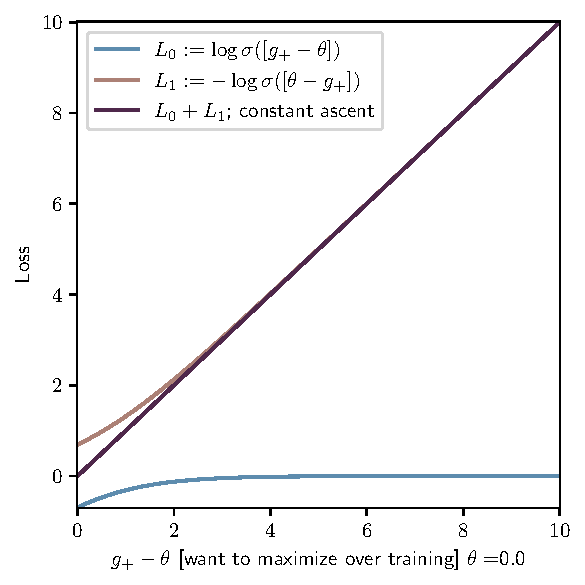
\includegraphics[width=0.32\linewidth]{FFA/memo/code//../plots/lfunc0}
\label{fig:lfunc0}
}
\qquad
\subfloat[FFA Time to Position]{
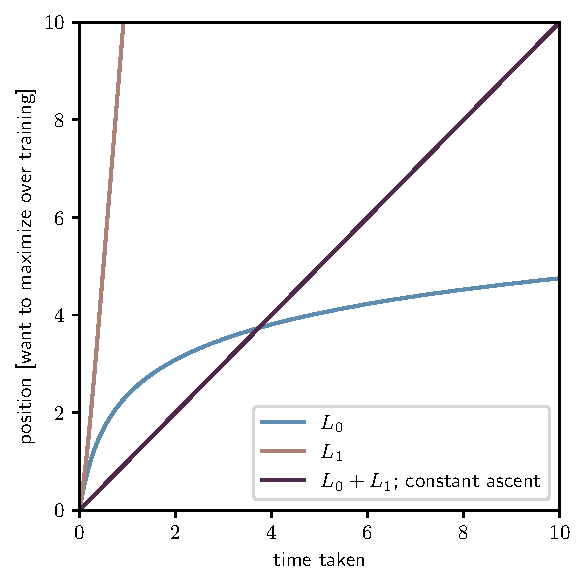
\includegraphics[width=0.32\linewidth]{FFA/memo/code//../plots/lfunc20}
\label{fig:lfunc20}
}
\qquad
\subfloat[FFA Loss over Time]{
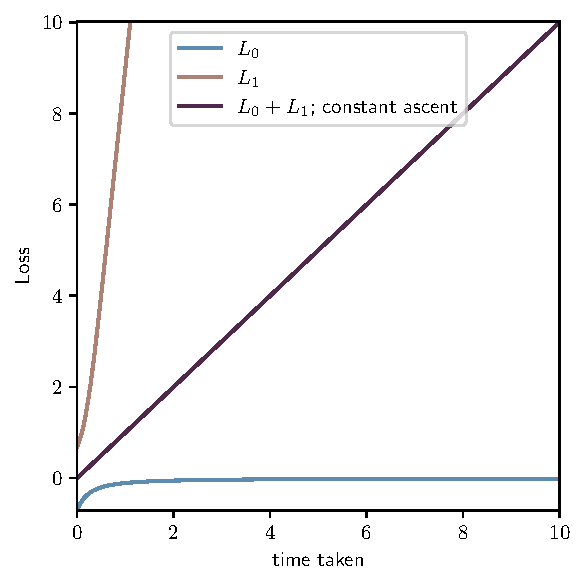
\includegraphics[width=0.32\linewidth]{FFA/memo/code//../plots/lfunc30}
\label{fig:lfunc30}
}

\end{figure}


\begin{figure}[htpb]
\centering

\subfloat[FFA Loss]{
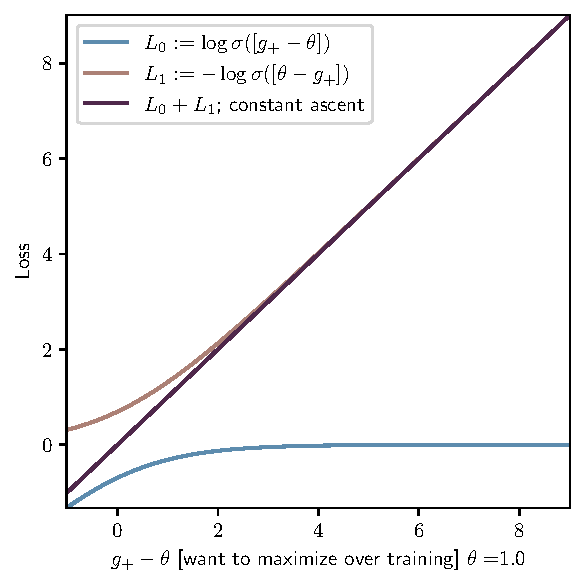
\includegraphics[width=0.32\linewidth]{FFA/memo/code//../plots/lfunc1}
\label{fig:lfunc1}
}
\qquad
\subfloat[FFA Time to Position]{
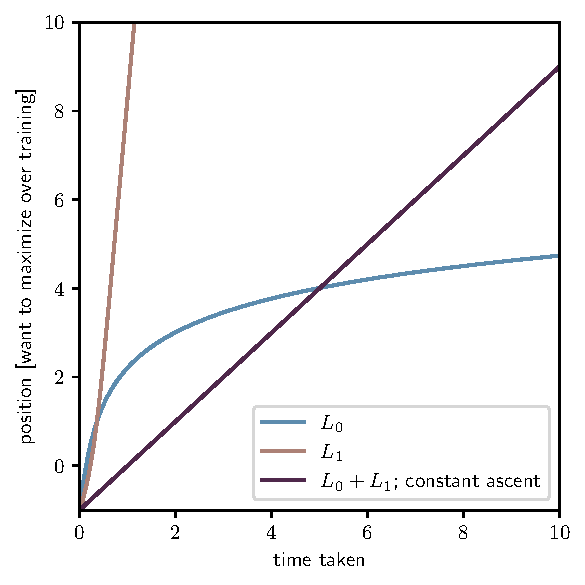
\includegraphics[width=0.32\linewidth]{FFA/memo/code//../plots/lfunc21}
\label{fig:lfunc21}
}
\qquad
\subfloat[FFA Loss over Time]{
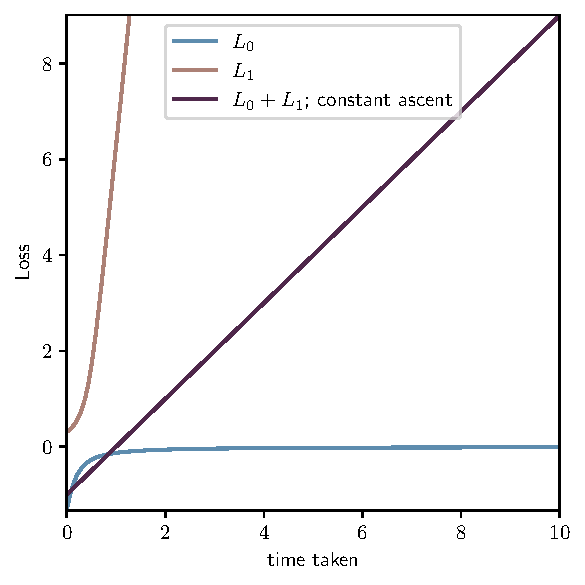
\includegraphics[width=0.32\linewidth]{FFA/memo/code//../plots/lfunc31}
\label{fig:lfunc31}
}

\end{figure}


\begin{figure}[htpb]
\centering

\subfloat[FFA Loss]{
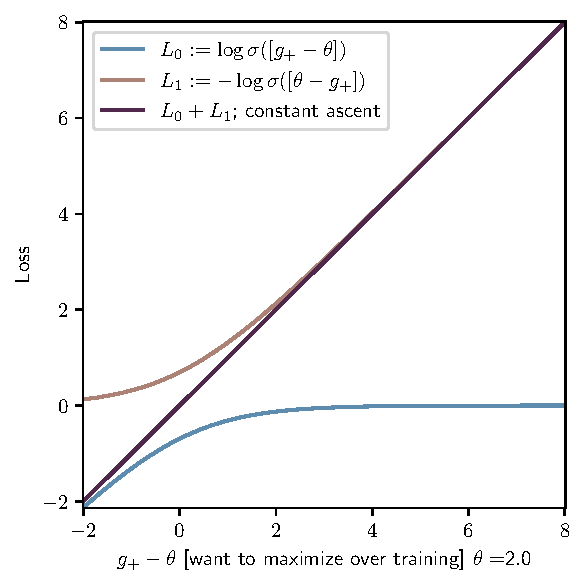
\includegraphics[width=0.32\linewidth]{FFA/memo/code//../plots/lfunc2}
\label{fig:lfunc2}
}
\qquad
\subfloat[FFA Time to Position]{
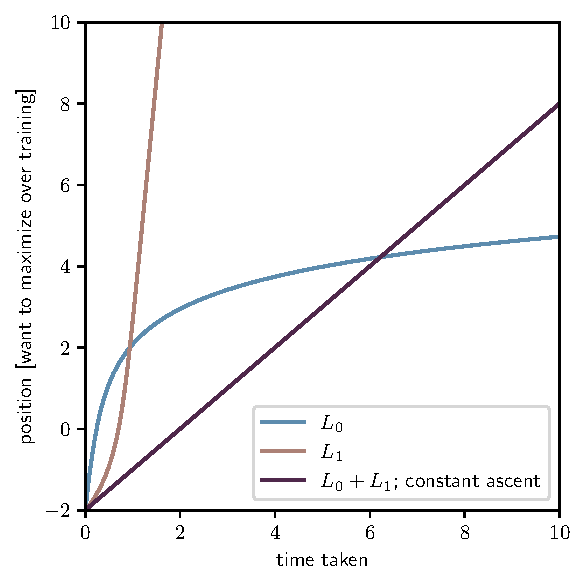
\includegraphics[width=0.32\linewidth]{FFA/memo/code//../plots/lfunc22}
\label{fig:lfunc22}
}
\qquad
\subfloat[FFA Loss over Time]{
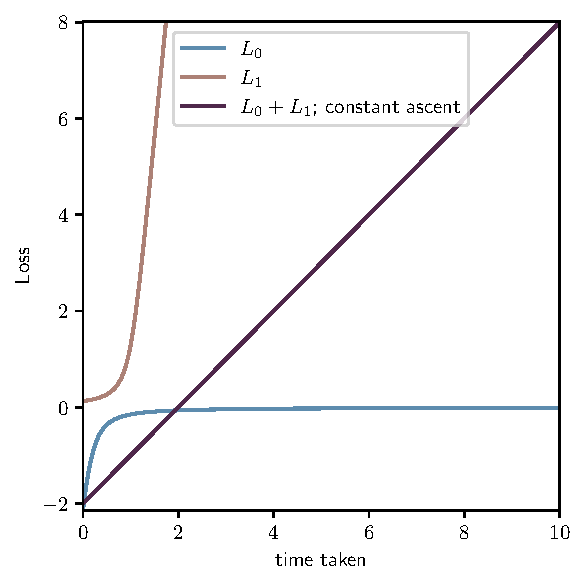
\includegraphics[width=0.32\linewidth]{FFA/memo/code//../plots/lfunc32}
\label{fig:lfunc32}
}

\end{figure}

$L_0$ is clearly a loss that learns slowly near to the supposed minima, while $L_1$ is a loss that learns slowly at the start.
Notice $L_0 + L_1 = x$, so a switch between the two during learning ($L_0 \rightarrow L_1$) should be best.
Plots for 3 thresholds (0.0, 1.0, 2.0) are shown. While (b) and (c) require integration against a somewhat inconsistent setpoint, (a) allows straightforward comparison.
The primary takeway: $L_0$ loss is slow but maintains a bounded loss, while $L_1$ loss is fast but easily explodes.
	
\section{Results}
The MNIST (numbers) dataset \cite{MNIST} was used to test the FFA losses.
A 784x800x10 network was used in all cases with consistent batching rates.
The learning rate was increased along with the batch size throughout training.
FFA0 uses the FFA $L_0$ loss and FFA1 uses the FFA $L_1$ loss.
FFA nets marked as adj., use the adjusted loss functions, where the $\ln[\cdots]$ is replaced with $\ln[1 + \cdots]$,to prevent the loss from exploding.
The FFA was trained similar to a DNN (each layer at a time instead of each layer in parallel) to eliminate differences.
\begin{alignat}{2}
L_0 = -\E[\ln[1 + \sigma(g_+-\theta)\oplus\sigma(\theta-g_-)]] \\
L_1 = \E[\ln[1 + \sigma(\theta-g_+)\oplus\sigma(g_--\theta)]]
\end{alignat}
\begin{tabular}{ c|c c c c c|c c}
Net & Opt & Epochs & Rate & Start & Final & Time[m:s] & Accuracy \\
\hline
DNN\_base   & ASGD & 400 & 1e-3 & 50 & 60000 & 0:24 & 97.73\% \\
FFA0       & ASGD & 400 & 1e-3 & 50 & 60000 & 1:22 & NAN \\
FFA1       & ASGD & 400 & 1e-3 & 50 & 60000 & 1:14 & NAN \\
adj\_FFA0\_0 & ASGD & 400 & 1e-3 & 50 & 3200 & 4:23 & 50.67\% \\
adj\_FFA0\_1 & ASGD & 400 & 1e-3 & 50 & 60000 & 1:23 & 49.80\% \\
adj\_FFA1\_0 & ASGD & 400 & 1e-3 & 50 & 3200 & 4:23 & 19.24\% \\
adj\_FFA1\_1 & ASGD & 400 & 5e-4 & 50 & 3200 & 4:23 & 24.84\% \\
adj\_FFA1\_2 & ASGD & 400 & 1e-3 & 50 & 60000 & 1:21 & 21.38\% \\
adj\_FFA0\_2 & Adam & 400 & 1e-3 & 50 & 60000 & 1:13 & NAN \\
adj\_FFA1\_3 & Adam & 400 & 1e-3 & 50 & 60000 & 1:18 & NAN \\
\end{tabular} \\
	
	
	
Start and Final are the batch sizes used at the start and end of training.
Clearly, the FFA $L_0$ loss performs better, but nowhere near as well as standard backpropagation.\\
	
\section{Appendix}
\sfig{FFA/memo/plots/DNN}{DNN Baseline}
\sfig{FFA/memo/plots/pFFA0}{FFA0}
\sfig{FFA/memo/plots/pFFA1}{FFA1}
\sfig{FFA/memo/plots/FFA0_0}{adj\_FFA0\_0}
\sfig{FFA/memo/plots/FFA0_1}{adj\_FFA0\_1}
\sfig{FFA/memo/plots/FFA1_0}{adj\_FFA1\_0}
\sfig{FFA/memo/plots/FFA1_1}{adj\_FFA1\_1}
\sfig{FFA/memo/plots/FFA1_2}{adj\_FFA1\_2}
\sfig{FFA/memo/plots/FFA0_2}{adj\_FFA0\_2}
\sfig{FFA/memo/plots/FFA1_3}{adj\_FFA1\_3}
	
	
\section{References}
\bibliography{References}
\end{document}